\documentclass{article}

\usepackage{../mathclub}

\title{Information and Coding Theory}
\author{}
\date{February 14, 2022}

\begin{document}

\section{Introduction}

Welcome to Math Club week 7!
A few weeks ago, we took a look at cryptography, which involved Alice and Bob sending messages to one another in such a way that no eavesdropper could read such messages.
There, we assumed that there were no physical issues with transmitting such messages: if they were sent in a certain form, they would necessarily arrive looking exactly the same.
Today, we will take a look at information theory and coding theory, which concern sending messages across \textbf{noisy channels}, or communication channels where the data sent may be potentially corrupted along the way. 
For example, a telephone line is an example of a noisy channel because when you talk to your friend on the phone, their voice may not sound crystal-clear as though they stood next to you.

The task at hand is to find a way to add extra information to your messages so that even if some of the data gets lost along the way, the recipient can still understand what you're trying to say. 
\textbf{Information theory} concerns itself with the theoretical limitation of this task while \textbf{coding theory} provides some actual ways of encoding messages to help protect from this data loss.

We will suppose for today that all of our messages are just binary strings: collections of 1s and 0s.

\section{Basic Error Correcting Codes}

\subsection{Repitition codes}

Suppose Alice wanted to send the message \(s = \texttt{0010110}\) to Bob across a noisy channel, where some of the bits (binary digits) might get flipped \((0\mapsto 1\textrm{ or }1\mapsto 0)\) along the way.
Suppose the chances of a bit flipping are \(f=0.1\).
One way might be to use a \textbf{repitition code} such as \(R_3\), in which we simply repeat each bit three times.
After sending our encoded message \(t = \texttt{000 000 111 000 111 111 000}\) across the noisy channel, we get the result
\[n = \texttt{000 001 111 000 010 111 000}.\]
Knowing Alice encoded with \(R_3\), Bob might deduce that the message is \(s' = \texttt{0010010}\), where he simply took the majority as the intended bit. 
Of course, Bob got unlucky here because two bits corresponding to the second 1 got flipped, so he incorrecly thought this was a 0.

\begin{exercise}
    In the example above, compute the probability that the message \(s\) makes its way through the channel without getting any bits flipped. Assume we have not encoded it in any way, but just sent \(s\) alone.
\end{exercise}

\begin{exercise}
    In the example given above, what is the probability that Bob would be able to accurately decode the message using his strategy of taking the majority?
\end{exercise}

\begin{exercise}
    Devise a way of encoding a message with higher probability of successful decoding than the \(R_3\) code.
    Can you devise a way that is \textit{not} a repitition code?
\end{exercise}

\begin{exercise}
    What is the probability Bob could accurately decode the message in the example above if we instead used \(R_5\), which sends the message \(t = \texttt{00000 00000 11111 00000 11111 11111 00000}\)?
\end{exercise}

\begin{exercise}
    \begin{enumerate}
        \item[(a)] Show that the probability of error of \(R_N\), the repitition code with \(N\) repititions is 
        \[p_b = \sum_{n=(N+1)/2}^N\binom{N}{n}f^n(1-f)^{N-n},\]
        for odd \(N\), where \(f\) is the probability of a bit flip across the noisy channel.
        \item[(b)] Assuming \(f=0.1\), which of the terms in the sum is the largest?
        How much larger is it than the second-largest term?
        \item[(c)] Using \textbf{Stirling's approximation}
        \[x! \approx x^xe^{-x}\sqrt{2\pi x}\]
        to approximate \(\binom{N}{n}\) in the largest term, find the approximate probability of error in the repitition code with \(N\) repititions.
        \item[(d)] Assuming \(f=0.1\), find how many repititions are required to get the probability of error down to \(10^{-15}\).
    \end{enumerate}
    This exercise tells us that in order to build a gigabyte disk drive with good enough reliability (\(10^{-15}\) chance of error), we would need \(k\) gigabytes of data if \(f=0.1\), where \(k\) is the answer to part (4). 
    This says that maybe the repitition code isn't the most efficient way to do this.
\end{exercise}

\subsection{Block Codes}

Instead of just repeating a bunch of bits, a \textbf{block code} takes a message \(s\) of length \(K\) and adds some information, turning it into a message \(t\) of length \(N\), where \(N>K\).
The extra \(N-K\) bits are called \textbf{parity check bits}.
One type of block code is the \textbf{(7,4) Hamming Code}, named for Richard Hamming, an important figure in the field of information theory.
This code transmits \(N=7\) bits of information for every \(K=4\) bits of message.
Suppose we wanted to send \(s = \texttt{1000}\).
\begin{center}
    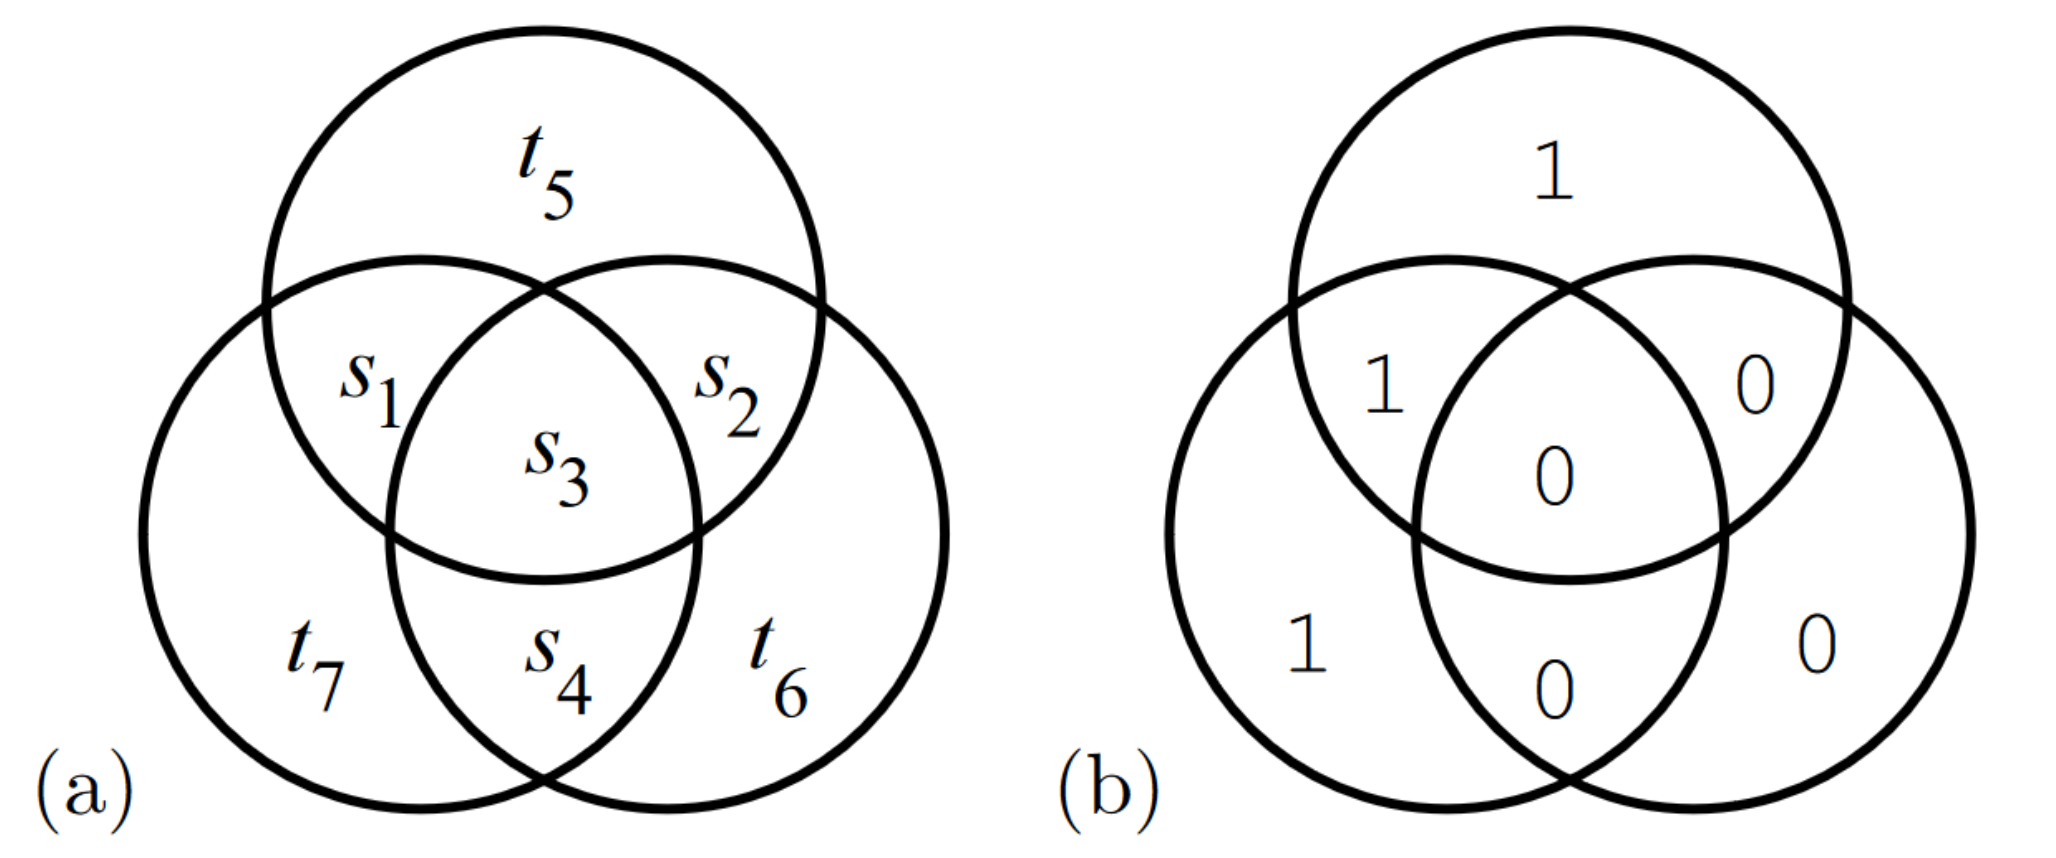
\includegraphics[scale=0.15]{Pics/hamming74.png}
\end{center}
From \(s = s_1s_2s_3s_4\), we generate the message \(t = s_1s_2s_3s_4t_5t_6t_7\), where the encoding is done so that the parity (odd or even) of the sum of the bits within each circle is even.
We can ensure this happens by choosing the parity check bits \(t_5t_6t_7\) in a particular way.

\begin{exercise}
    Generate the value of \(t\) for the following values of \(s\): \(s = \texttt{0000}\), \(s = \texttt{1111}\), \(s = \texttt{1010}\), \(s = \texttt{0111}\), \(s = \texttt{1000}\).
\end{exercise}

Since this is more complicated than the repitition codes, it stands to reason that decoding the (7,4) Hamming code is more complicated.
Remember that when sent across the noisy channel, \textit{any} of the bits of \(t\) might have been flipped, including the parity check bits.
The trick is to compute a 3-bit \textbf{syndrome} as follows:
Write the message you recieve in the Venn diagram as above.
Then your syndome \(z = z_1z_2z_3\) checks whether the three circles are satisfied (parity-wise) or not.
More precisely, \(z_1=1\) if the top circle violates the partiy rules and 0 otherwise. \(z_2\) is the same but for the circle on the right, and \(z_3\) is for the circle on the left.
This allows us to check which bit has been flipped and unflip it so that we recover the original message.
Given the message \(r_1r_2r_3r_4r_5r_6r_7\), we use the table:
\begin{table}[h!]
    \begin{center}
        \begin{tabular}{l|llllllll}
            Syndome \(z\) &\texttt{000} &\texttt{001} &\texttt{010} &\texttt{011} &\texttt{100} &\texttt{101} &\texttt{110} &\texttt{111} \\\hline
            Unflip this bit & none & \(r_7\) & \(r_6\) & \(r_4\) & \(r_5\) & \(r_1\) & \(r_2\) & \(r_3\)
        \end{tabular}
    \end{center}
\end{table}

\begin{exercise}
    Decode the following recieved strings: \(r = \texttt{1101011}\), \(r = \texttt{0110110}\), \(r = \texttt{0100111}\), \(r = \texttt{1111111}\).
\end{exercise}

\begin{exercise}
    Does the (7,4) Hamming code detect any single-bit-flip error? 
    What about if there were two bits flipped by the noisy channel? 
\end{exercise}

\begin{exercise}
    Might there be a (14,8) code which can detect any two errors?
\end{exercise}

\begin{exercise}
    Devise your own error-correcting code other than a repitition code and the (7,4) Hamming code and a decoding algorithm for it.
    Compute the probability of error.
    Don't worry if it's not as efficient or successful as the ones we've seen.
\end{exercise}

\begin{exercise}
    Devise a code that can correct any two errors in the message.
    Prove that this is indeed the case.
\end{exercise}

\end{document}